\section{Mengen Terme und Gleichungen}
\subsection{Mengen}
\textbf{Einführungsfrage}: Welche Arten von Zahlen kennen Sie?

Bei gewissen Fragestellungen ist oft klar, dass man sich nur für eine bestimmte Art von Zahlen interessiert. Wenn man beispielsweise nach einer Streckenlänge fragt, kommen nur positive Zahlen infrage. Bei den Schulnoten hingegen kommen nur die Zahlen \(1, 1.5, 2, 2.5, \ldots\) bis \(6\) infrage. Für diese Fälle wurde der Begriff der Menge eingeführt.

\begin{definition}
    {Zahlenmenge}{}
    Eine \textbf{Zahlenmenge} \(M\) ist eine Zusammenfassung von bestimmten Zahlen.

    Gehört eine Zahl \(x\) zur Zahlenmenge \(M\), so sagt man, \(x\) ist \textbf{ein Element} der Menge \(M\) und schreibt dafür
    \[
        x \in M.
    \]
    Gehört eine Zahl \(x\) nicht zu einer Menge \(M\), so schreibt man
    \[
        x \notin M.
    \]

    Wenn eine Menge keine Elemente beinhaltet, spricht man von der leeren Menge
    \[
        \emptyset \qquad \text{oder} \qquad \{\}.
    \]

\end{definition}

Am einfachsten ist es wohl, wenn man sich eine Zahlenmenge als einen Sack vorstellt, der gewisse Zahlen enthält. Die leere Menge ist dann gewissermassen ein leerer Sack.

Wenn eine Menge nur wenige Zahlen enthält, kann sie durch \textit{Aufzählen} ihrer Elemente angegeben werden. Dafür schreibt man die Liste der Elemente in geschweiften Klammern. Die Menge der Schulnoten wäre dann
\[
    \{1, 1.5, 2, 2.5, \ldots, 6\}.
\]

Für Mengen mit vielen oder gar unendlich vielen Elementen ist die aufzählende Schreibweise ungünstig. Solche Mengen werden in der sogenannten \textit{beschreibenden Form} angegeben. Die Menge der Schulnoten wäre dann
\[
    \{x \mid 1 \leq x \leq 6,\; x \text{ ist ein Vielfaches von } 0.5\}.
\]

Der senkrechte Strich ist dabei eine Abkürzung für \enquote{mit der Eigenschaft, dass}.

\subsubsection{Wichtige Zahlenmengen}
Die natürlichen Zahlen sind jene Zahlen, die man beim Zählen verwendet:
\begin{definition}{Natürliche Zahlen}{natuerlichezahlen}
    Die Menge \(\mathbb{N}\) der natürlichen Zahlen ist die Menge
    \[ \N = \{1, 2, 3, 4, 5, \ldots\} \]
\end{definition}
Die Gemeinschaft der Mathematiker ist sich uneins, ob die Zahl \(0\) auch zu den natürlichen Zahlen gehören soll oder nicht. Bei uns wird sie standardmässig nicht dazugehören. Falls wir die Null benötigen, können wir die Zahlenmenge \(\mathbb{N}_0 = \{0, 1, 2, 3, 4, 5, \ldots\}\) betrachten.

\begin{definition}{Die ganzen Zahlen}{}
    Die Menge \(\mathbb{Z}\) der ganzen Zahlen ist definiert durch
    \[
        \mathbb{Z} = \{\ldots, -3, -2, -1, 0, 1, 2, 3, \ldots\}.
    \]

    Oder in beschreibender Form
    \[
        \mathbb{Z} = \{x \mid x \in \mathbb{N}_0 \text{ oder } -x \in \mathbb{N}\}.
    \]

    (Die beschreibende Form liest man so: \textit{\(\mathbb{Z}\) ist die Menge aller \(x\) mit der Eigenschaft, dass \(x\) in der Menge \(\mathbb{N}_0\) oder \(-x\) in der Menge \(\mathbb{N}\) liegt}.)
\end{definition}

\begin{definition}
    {Die rationale Zahlen}{}
    Das Resultat einer Division von zwei ganzen Zahlen nennt man einen (gewöhnlichen) Bruch.

    Die Menge \(\mathbb{Q}\) der rationalen Zahlen ist die Menge aller Brüche.
    \[
        \mathbb{Q}
        =
        \left\{
        \frac{a}{b}
        \;\middle|\;
        a \in \mathbb{Z}
        \text{ und }
        b \neq 0 \in \mathbb{Z}
        \right\}
    \]
\end{definition}

\textbf{Die reellen Zahlen \(\R\) }

Wenn Sie nun der Meinung sind, dass es jenseits der Brüche keine weiteren Zahlen gibt, sind Sie in bester Gesellschaft: Pythagoras (um 510 v.\,Chr. gestorben) war überzeugt, dass es gar keine anderen Zahlen als Brüche geben kann.

Als einer der Ersten hat wohl Hippasos von Metapont (ca.\ 500 v.\,Chr.) entdeckt, dass es Zahlen gibt, die sich nicht als Bruch schreiben lassen. Solche Zahlen nennt man auch \textit{irrational}. Zusammen mit den rationalen Zahlen bilden sie die Menge der reellen Zahlen:
\begin{definition}
    {Die reellen Zahlen \(\R\)}{}
    Die Menge \(\mathbb{R}\) der reellen Zahlen besteht aus allen rationalen und irrationalen Zahlen.
\end{definition}
Vielleicht haben Sie gemerkt, dass wir gar nicht genau festgelegt haben, was denn irrationale Zahlen sind. Eine genaue Definition der reellen Zahlen ist aber gar nicht so einfach. Siehe vielleicht später im Schwerpunktfach AM\dots

Wenn nichts anderes erwähnt wird, werden wir in der Mittelschule immer mit reellen Zahlen arbeiten. Diese können auf der sogenannten Zahlengerade angesiedelt werden: Jeder Zahl entspricht ein Punkt auf der Zahlengerade und umgekehrt.

\begin{center}
    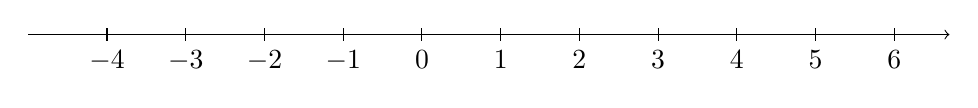
\begin{tikzpicture}
        \draw[->] (-5,0) -- (6.7,0);
        \foreach \x in {-4,-3,...,6} {
                \draw (\x,0.08) -- (\x,-0.08) node[below] {\(\x\)};
            }
    \end{tikzpicture}
\end{center}

Weitere Zahlenmengen:
\[
    \mathbb{R}^{+}
    =
    \{x \in \mathbb{R} \mid x > 0\}
    \qquad
    \text{\enquote{positive reelle Zahlen}}
\]

\[
    \mathbb{R}^{-}_{0}
    =
    \{x \in \mathbb{R} \mid x \leq 0\}
    \qquad
    \text{\enquote{negative reelle Zahlen und Null}}
\]

analog \(\mathbb{Z}^{-}\), \(\mathbb{Q}^{+}_{0}\), usw.



\textbf{\textit{Rational oder irrational?}}

Woran erkennt man eigentlich, ob eine Zahl rational ist (also in \(\mathbb{Q}\) liegt)? Das ist ganz einfach! Die Dezimaldarstellung von Brüchen ist entweder endlich oder periodisch.

\begin{itemize}
    \item \(2.423\) ist eine rationale Zahl, weil die Dezimaldarstellung endlich ist
          \[
              \left(2.423 = \frac{2423}{1000}\right).
          \]

    \item \(2.753753753753753\ldots = 2.\overline{753}\) ist eine rationale Zahl, weil die Dezimaldarstellung periodisch ist
          \[
              \left(2.\overline{753} = \frac{2751}{999}\right).
          \]
          (Wie findet man wohl den dazugehörigen Bruch?)

    \item \(1.234567891011121314\ldots\) ist eine irrationale Zahl, weil sie weder endlich noch periodisch ist.
\end{itemize}

Der letzte Punkt tönt einfacher als er ist: Schliesslich kennt man bei einer Zahl wie \(\sqrt{2}\) nicht alle unendlich vielen Ziffern nach dem Dezimalpunkt. Bloss weil sich in den ersten paar Milliarden kein sich wiederholendes Muster zeigt, heisst das noch lange nicht, dass in der darauffolgenden Unendlichkeit kein solches auftreten wird.

Mehr zu diesem Thema werden wir im letzten Teilkapitel besprechen \dots

\clearpage

\begin{ueb}
    {Übungen zu den wichtigen Zahlenmengen}{zahlenmengen}

    \begin{enumerate}
        \item Kreuzen Sie an, in welchen der angegebenen Zahlenmengen die Zahlen enthalten sind. Tipp: Wir werden später sehen, dass \(\sqrt{5}\) eine irrationale Zahl ist.

              \[
                  \begin{array}{c|c|c|c|c|c|c|c|c|c|c}
                                   & \dfrac{2}{5}   & 7               & -1.5      & -\dfrac{8}{4} & \sqrt{5} & \sqrt{16}
                                   & 1.4 \cdot 10^3 & 2.04 \cdot 10^2 & \sqrt{-5} & -\sqrt{5}                                       \\ \hline
                      \mathbb{N}   &                &                 &           &               &          &           &  &  &  & \\ \hline
                      \mathbb{Z}   &                &                 &           &               &          &           &  &  &  & \\ \hline
                      \mathbb{Q}   &                &                 &           &               &          &           &  &  &  & \\ \hline
                      \mathbb{Q}^- &                &                 &           &               &          &           &  &  &  & \\ \hline
                      \mathbb{R}   &                &                 &           &               &          &           &  &  &  &
                  \end{array}
              \]

        \item
              Beantworten Sie die Frage oder beurteilen Sie, ob die Aussage wahr oder falsch ist.

              \begin{enumerate}
                  \item Sind die negativen gewöhnlichen Brüche in \(\mathbb{Q}\) enthalten?
                  \item Jede natürliche Zahl liegt auch in \(\mathbb{Z}\).
                  \item Eine natürliche Zahl gehört nicht zu \(\mathbb{Q}\), weil sie ja schon in \(\mathbb{N}\) ist.
                  \item Liegen alle Dezimalbrüche in \(\mathbb{Q}\)?
                  \item Gehört jede Zahl in \(\mathbb{Q}\) auch zu \(\mathbb{R}\)?
              \end{enumerate}
        \item Beschreiben Sie in Worten, um welche Zahlen es sich handelt.

              \begin{enumerate}
                  \item \(\mathbb{Z}\) ohne \(\mathbb{N}\)
                  \item \(\mathbb{Z}\) ohne \(\{-1,-2,-3,\ldots\}\)
                  \item \(\mathbb{Q}^{+}\) ohne \(\{-1,-2,-3,\ldots\}\)
              \end{enumerate}
        \item Die folgenden Mengen sind in beschreibender Form angegeben. Geben Sie die Menge in aufzählender Form an.

              Zum Beispiel
              \[
                  \{n \in \mathbb{N} \mid 2n < 10\} = \{1,2,3,4\}.
              \]

              \begin{enumerate}
                  \item \(A = \{n \in \mathbb{N} \mid n \text{ ist ein Teiler von } 36\}\)
                  \item \(B = \{n \in \mathbb{N} \mid n < 10 \text{ und } n = 2k \text{ für eine Zahl } k \in \mathbb{N}\}\)
                  \item \(C = \{n \in \mathbb{N} \mid n^2 \leq 100\}\)
                  \item \(D = \{x \in \mathbb{Z} \mid -3 \leq x - 5 \leq 3\}\)
              \end{enumerate}

        \item Die folgenden Mengen sind in aufzählender Form angegeben. Geben Sie die Menge in beschreibender Form an.

              \begin{enumerate}
                  \item \(A = \{1,8,27,64,125\}\)
                  \item \(B = \{3,4,5,6,7,8,9,10\}\)
                  \item \(C = \{1,3,5,7,9,11\}\)
                  \item \(D = \{1,2,3,4,6,12\}\)
              \end{enumerate}
        \item Challenge:
              \begin{enumerate}
                  \item Erklären Sie, wie man den Bruch für die Zahl \(x = 2.\overline{753}\) findet. Tipp: Betrachten Sie die Zahl \(1000\cdot x\) und die Zahl \(x\) und berechnen Sie damit die Zahl \(999\cdot x\).
                  \item Finden Sie einen Bruch für die Zahl \(x = 1.234\overline{34}\).
              \end{enumerate}
    \end{enumerate}


\end{ueb}



% \clearpage
\emph{Lösungen:}

\begin{enumerate}
    \item
          \[
              \begin{array}{c|c|c|c|c|c|c|c|c|c|c}
                               & \dfrac{2}{5}   & 7               & -1.5      & -\dfrac{8}{4} & \sqrt{5} & \sqrt{16}
                               & 1.4 \cdot 10^3 & 2.04 \cdot 10^2 & \sqrt{-5} & -\sqrt{5}                            \\ \hline
                  \mathbb{N}   &                & \times          &           &               &          & \times
                               & \times         & \times          &           &                                      \\ \hline
                  \mathbb{Z}   &                & \times          &           & \times        &          & \times
                               & \times         & \times          &           &                                      \\ \hline
                  \mathbb{Q}   & \times         & \times          & \times    & \times        &          & \times
                               & \times         & \times          &           &                                      \\ \hline
                  \mathbb{Q}^- &                &                 & \times    & \times        &          &
                               &                &                 &           &                                      \\ \hline
                  \mathbb{R}   & \times         & \times          & \times    & \times        & \times   & \times
                               & \times         & \times          &           & \times
              \end{array}
          \]

    \item
          \begin{enumerate}
              \item Ja.
              \item Wahr.
              \item Falsch.
              \item Wahr.
              \item Ja.
          \end{enumerate}

    \item
          \begin{enumerate}
              \item Die ganzen Zahlen kleiner oder gleich \(0\).
              \item Die nichtnegativen ganzen Zahlen, also \(\mathbb{N}_0\).
              \item Die positiven rationalen Zahlen, also \(\mathbb{Q}^+\).
          \end{enumerate}

    \item
          \begin{enumerate}
              \item \(A = \{1,2,3,4,6,9,12,18,36\}\)
              \item \(B = \{2,4,6,8\}\)
              \item \(C = \{1,2,3,4,5,6,7,8,9,10\}\)
              \item \(D = \{2,3,4,5,6,7,8\}\)
          \end{enumerate}

    \item
          \begin{enumerate}
              \item \(A = \{n^3 \mid n \in \mathbb{N},\ n \leq 5\}\)
              \item \(B = \{n \in \mathbb{N} \mid 3 \leq n \leq 10\}\)
              \item \(C = \{n \in \mathbb{N} \mid n < 12 \text{ und } n \text{ ungerade}\}\)
              \item \(D = \{n \in \mathbb{N} \mid n \text{ ist ein Teiler von } 12\}\)
          \end{enumerate}

    \item \begin{enumerate}
              \item \(\frac{917}{333}\)
              \item \(\frac{611}{495}\)
          \end{enumerate}
          %       \begin{enumerate}
          %           \item
          %                 \[
          %                     1000x = 2753.\overline{753},
          %                     \qquad
          %                     x = 2.\overline{753}
          %                 \]
          %                 \[
          %                     999x = 2751
          %                     \qquad\Longrightarrow\qquad
          %                     x = \frac{2751}{999}
          %                     = \frac{917}{333}.
          %                 \]

          %           \item
          %                 \[
          %                     100000x - 1000x = 122200
          %                 \]
          %                 \[
          %                     99000x = 122200
          %                     \qquad\Longrightarrow\qquad
          %                     x = \frac{122200}{99000}
          %                     = \frac{611}{495}.
          %                 \]
          % \end{enumerate}
\end{enumerate}



\clearpage
\subsubsection{Mengenoperationen und Teilmengen}
Vergleicht man die Elemente der Mengen \(\mathbb{Z}\) und \(\mathbb{N}\), so stellt man fest, dass alle Elemente von \(\mathbb{N}\) auch in \(\mathbb{Z}\) enthalten sind. Man sagt dann, dass \(\mathbb{N}\) eine Teilmenge von \(\mathbb{Z}\) ist:

\begin{definition}{Teilmenge}{teilmenge}
    Eine Menge \(A\) heisst \textit{Teilmenge} einer Menge \(B\), wenn alle Elemente von \(A\) auch in der Menge \(B\) liegen.

    Schreibweise:
    \[
        A \subset B
    \]

    \begin{center}
        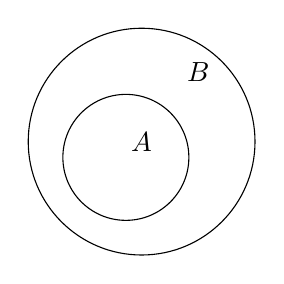
\begin{tikzpicture}[scale=0.8]
            \draw (0,0) circle (1.8);
            \draw (-0.25,-0.25) circle (1.0);
            \node at (0,0) {\(A\)};
            \node at (0.9,1.1) {\(B\)};
        \end{tikzpicture}
    \end{center}
\end{definition}

Bemerkung: Ist \(A\) keine Teilmenge von \(B\), schreibt man
\[
    A \not\subset B.
\]

\textbf{Beispiel:}
\[
    \mathbb{Z} \subset \mathbb{R}.
\]

\begin{definition}{Schnittmenge}{schnittmenge}
    Die \textit{Schnittmenge} der Mengen \(A\) und \(B\) ist diejenige Menge, die alle Elemente enthält, welche in \(A\) und in \(B\) enthalten sind.

    Schreibweise für Schnittmengen:
    \[
        A \cap B
    \]

    Es gilt:
    \[
        A \cap B = \{x \mid x \in A \text{ und } x \in B\}.
    \]

    \begin{center}
        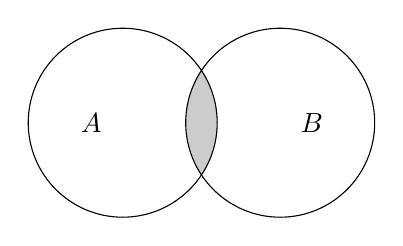
\begin{tikzpicture}
            \begin{scope}
                \clip (-1,0) circle (1.2);
                \fill[gray!40] (1,0) circle (1.2);
            \end{scope}
            \draw (-1,0) circle (1.2);
            \draw (1,0) circle (1.2);
            \node at (-1.4,0) {\(A\)};
            \node at (1.4,0) {\(B\)};
        \end{tikzpicture}
    \end{center}
\end{definition}

\textbf{Beispiel einer Schnittmenge:}
\[
    \{\text{Primzahlen}\}
    \cap
    \{\text{natürliche Zahlen kleiner als } 10\}
    =
    \{2,3,5,7\}.
\]

\begin{definition}{Vereinigungsmenge}{vereinigungsmenge}
    Die \textit{Vereinigungsmenge} der Mengen \(A\) und \(B\) ist diejenige Menge, die alle Elemente enthält, die in der Menge \(A\) oder \(B\) enthalten sind.

    Schreibweise für Vereinigungsmengen:
    \[
        A \cup B
    \]

    Es gilt:
    \[
        A \cup B = \{x \mid x \in A \text{ oder } x \in B\}.
    \]

    \begin{center}
        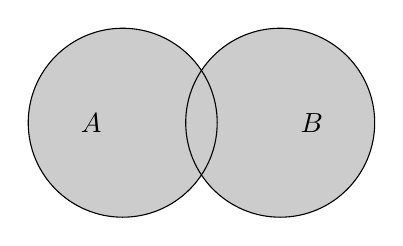
\begin{tikzpicture}
            \fill[gray!40] (-1,0) circle (1.2);
            \fill[gray!40] (1,0) circle (1.2);
            \draw (-1,0) circle (1.2);
            \draw (1,0) circle (1.2);
            \node at (-1.4,0) {\(A\)};
            \node at (1.4,0) {\(B\)};
        \end{tikzpicture}
    \end{center}
\end{definition}

\textbf{Beispiel einer Vereinigungsmenge:}
\[
    \{\text{Teiler von } 6\}
    \cup
    \{x \mid x \in \mathbb{N} \text{ und } 4 < x < 8\}
    =
    \{1,2,3,5,6,7\}.
\]

\begin{definition}{Differenzmenge}{differenzmenge}
    Die \textit{Differenzmenge} der Mengen \(A\) und \(B\) ist diejenige Menge, die alle Elemente enthält, die in der Menge \(A\), aber nicht in der Menge \(B\) enthalten sind.

    Schreibweise für Differenzmengen:
    \[
        A \setminus B
    \]

    Es gilt:
    \[
        A \setminus B
        =
        \{x \mid x \in A \text{ und } x \notin B\}.
    \]

    \begin{center}
        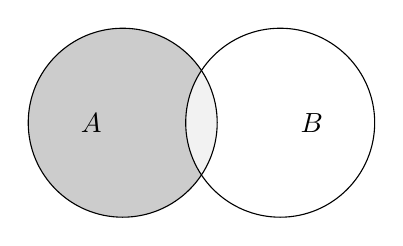
\begin{tikzpicture}
            \begin{scope}
                \clip (-1,0) circle (1.2);
                \fill[gray!40] (-1,0) circle (1.2);
                \fill[gray!10] (1,0) circle (1.2);
            \end{scope}
            \draw (-1,0) circle (1.2);
            \draw (1,0) circle (1.2);
            \node at (-1.4,0) {\(A\)};
            \node at (1.4,0) {\(B\)};
        \end{tikzpicture}
    \end{center}
\end{definition}

\textbf{Beispiel einer Differenzmenge:}
\[
    \{\text{Teiler von } 6\}
    \setminus
    \{\text{Primzahlen}\}
    =
    \{1,6\}.
\]

In Anwendungssituationen wird häufig nur ein beschränkter Bereich der reellen Zahlen betrachtet. Wenn die Variable \(v\) die Schnelligkeit eines Teilchens in \(\mathrm{m/s}\) beschreibt, so ist \(v\) eine reelle Zahl zwischen Null und der Lichtgeschwindigkeit \(c \cong 299'792'458\).

In der Sprache der Mathematik würde man sagen: \(v\) liegt im \textbf{Intervall} \([0,c]\).

\begin{definition}{Intervalle}{intervalle}
    \textbf{Intervalle} sind Mengen von reellen Zahlen zwischen zwei Grenzen. Je nachdem, ob die eckigen Klammern nach innen oder aussen zeigen, gehören die Grenzen zur Menge oder nicht. Für \(a<b\) gilt:
    \[
        \begin{aligned}
            [a,b]                                                & = \{x \in \mathbb{R} \mid a \leq x \leq b\}, \\
            ]a,b[                                                & = \{x \in \mathbb{R} \mid a < x < b\},       \\
            [a,b[   &= \{x \in \mathbb{R} \mid a \leq x < b\},\\
                    ]a,b] & = \{x \in \mathbb{R} \mid a < x \leq b\}.
        \end{aligned}
    \]
\end{definition}

\textbf{Speziell:} Man kann mit der Intervallschreibweise auch unbeschränkte Mengen angeben. Die Menge aller reellen Zahlen, die grösser oder gleich \(5\) sind, wäre zum Beispiel
\[
    M = [5,\infty[.
\]

Analog ist
\[
    ]-\infty,10[
\]
die Menge aller reellen Zahlen, die kleiner als \(10\) sind.

Oder im Extremfall:
\[
    \mathbb{R} = ]-\infty,\infty[.
\]

Merke: Bei \(\infty\) zeigt die Klammer immer gegen aussen.

\begin{bsp}
    {}{}
    \[ [-2, 2 [ \, \cap \, ]0, 3] = ? \]
    \vspace*{5 cm}
\end{bsp}































\clearpage

\begin{ueb}
    {Zu Mengenoperationen und Intervalle}{}
    \begin{enumerate}
        \item Setzen Sie für \(\diamond\) das richtige Zeichen
              \(\left(\in,\notin,\subset,\not\subset\right)\) ein.

              \begin{enumerate}
                  \item \(\mathbb{Z} \diamond \mathbb{Q}\)
                  \item \(\mathbb{Z} \diamond \mathbb{N}\)
                  \item \(-5 \diamond \mathbb{N}\)
                  \item \(-5 \diamond \mathbb{Q}\)
                  \item \(\{2,7\} \diamond \mathbb{N}\)
                  \item \(\{0,\pm1,\pm2,\pm3,\ldots\} \diamond \mathbb{Z}\)
              \end{enumerate}

        \item Gegeben sind die Mengen
              \[
                  A=\{11,13,15,17,18\}
                  \qquad\text{und}\qquad
                  B=\{10,12,13,14,16\}.
              \]
              Bestimmen Sie:

              \begin{enumerate}
                  \item \(A \cup B\)
                  \item \(A \cap B\)
                  \item \(A \setminus B\)
                  \item \(B \setminus A\)
                  \item \((A \setminus B)\cup(B \setminus A)\)
                  \item \((A \cup B)\setminus(A \cap B)\)
              \end{enumerate}

        \item Setzen Sie für \(\diamond\) das richtige Zeichen
              \(\left(\in,\notin,\subset,\not\subset\right)\) ein.

              \begin{enumerate}
                  \item \(b \diamond \{a,b,c,d,e,f\}\)
                  \item \(\{b\} \diamond \{a,b,c,d,e,f\}\)
                  \item \(\{b,d,g\} \diamond \{a,b,c,d,e,f\}\)
                  \item \(g \diamond \{a,b,c,d,e,f\}\)
                  \item \(\{a,b,c,d,e\} \diamond \{a,b,c\}\)
                  \item \(\{b,c,d,e\} \diamond \{b,c,d,e\}\)
              \end{enumerate}

        \item Beurteilen Sie, ob die Aussage wahr oder falsch ist.

              \begin{enumerate}
                  \item \((A \cup B) \subset B\)
                  \item \((A \cap B) \subset B\)
                  \item \(A \subset (A \cup B)\)
                  \item \(A \subset (A \cap B)\)
              \end{enumerate}
        \item Geben Sie die folgenden Mengen als ein Intervall an:

              \begin{enumerate}
                  \item \(A = \{x \in \mathbb{R} \mid -5 < x \leq 3\}\)
                  \item \(B = \{x \in \mathbb{R} \mid 1 < x < 2.5\}\)
                  \item \(C = \{x \in \mathbb{R} \mid x < 1\}\)
                  \item \(D = [-1,5] \cup [4,6[\)
                  \item \(E = [-1,5] \cap [4,6[\)
                  \item \(F = [-2,8] \setminus [5,9]\)
              \end{enumerate}
    \end{enumerate}
\end{ueb}


\emph{Lösungen:}
\begin{enumerate}
    \item
          \begin{enumerate}
              \item \(\mathbb{Z} \subset \mathbb{Q}\)
              \item \(\mathbb{Z} \not\subset \mathbb{N}\)
              \item \(-5 \notin \mathbb{N}\)
              \item \(-5 \in \mathbb{Q}\)
              \item \(\{2,7\} \subset \mathbb{N}\)
              \item \(\{0,\pm1,\pm2,\pm3,\ldots\} \subset \mathbb{Z}\)
          \end{enumerate}

    \item
          \begin{enumerate}
              \item \(A \cup B = \{10,11,12,13,14,15,16,17,18\}\)
              \item \(A \cap B = \{13\}\)
              \item \(A \setminus B = \{11,15,17,18\}\)
              \item \(B \setminus A = \{10,12,14,16\}\)
              \item \((A \setminus B)\cup(B \setminus A) = \{10,11,12,14,15,16,17,18\}\)
              \item \((A \cup B)\setminus(A \cap B) = \{10,11,12,14,15,16,17,18\}\)
          \end{enumerate}

    \item
          \begin{enumerate}
              \item \(b \in \{a,b,c,d,e,f\}\)
              \item \(\{b\} \subset \{a,b,c,d,e,f\}\)
              \item \(\{b,d,g\} \not\subset \{a,b,c,d,e,f\}\)
              \item \(g \notin \{a,b,c,d,e,f\}\)
              \item \(\{a,b,c,d,e\} \not\subset \{a,b,c\}\)
              \item \(\{b,c,d,e\} \subset \{b,c,d,e\}\)
          \end{enumerate}

    \item
          \begin{enumerate}
              \item Falsch.
              \item Wahr.
              \item Wahr.
              \item Falsch.
          \end{enumerate}

    \item
          \begin{enumerate}
              \item \(A = ]-5,3]\)
              \item \(B = ]1,2.5[\)
              \item \(C = ]-\infty,1[\)
              \item \(D = [-1,6[\)
              \item \(E = [4,5]\)
              \item \(F = [-2,5[\)
          \end{enumerate}
\end{enumerate}

\clearpage












\subsubsection{Rationale und irrationale Zahlen}

In diesem Abschnitt werden wir den Unterschied zwischen rationalen und irrationalen Zahlen genauer untersuchen. Dabei werden wir die folgenden drei Fragen diskutieren:
\begin{itemize}
    \item Wieso kann man jede periodische Dezimalzahl als Bruch schreiben?
    \item Wieso ist die Dezimaldarstellung einer rationalen Zahl entweder endlich oder periodisch?
    \item Wie kann man zeigen, dass eine Zahl wie \(\sqrt{2}\) irrational ist?
\end{itemize}

Die erste Frage haben Sie vielleicht bereits in der Übung \Cref{uebng:zahlenmengen} beantwortet: Durch geschicktes Rechnen kann man bei einer solchen Zahl zum Beispiel \( x = 2.\overline{753}\) die Nachkommastellen eliminieren. In diesem Fall rechnet man:
\[
    1000x = 2753.\overline{753},
    \qquad
    x = 2.\overline{753}
\]
Damit erhält man:
\[
    999x = 2751
    \qquad\Longrightarrow\qquad
    x = \frac{2751}{999}
    = \frac{917}{333}.
\]

Man kann sich leicht überlegen, dass man auf diese Weise jede periodische Zahl als Bruch darstellen kann.

Zur zweiten Frage:

\begin{LA}
    {Brüche haben eine periodische Dezimaldarstellung}{}
    Die folgenden Aufgaben sollen Ihnen helfen zu verstehen, wieso jeder Bruch eine periodische (oder endliche) Dezimaldarstelung hat.
    \begin{enumerate}
        \item Finden Sie die Dezimaldarstellung von \(\frac{1}{7}\), indem Sie schriftlich dividieren:
              \begin{align*}
                   & 1.00000 : 7 = 0.1\ldots \\
                   & 10                      \\
                   & \phantom{1}30
              \end{align*}
              \vspace*{2 cm}
        \item 	Wann beginnt sich die Dezimaldarstellung zu wiederholen? Wie viele verschiedene Reste kann es bei einer Division durch eine ganze Zahl \(n\) geben?
        \item 	Wieso ist die Dezimaldarstellung von \(\frac{1}{n}\) endlich oder periodisch? Wie lang kann die Periode sein?
    \end{enumerate}
\end{LA}












\clearpage

Nachdem wir die ersten beiden Fragen beantwortet haben, ist klar, dass die rationalen Zahlen genau die Zahlen sind, deren Dezimaldarstellung endlich oder periodisch ist. So kann man sich leicht eine irrationale Zahl denken. Zum Beispiel ist die Zahl \(1.234567891011121314\ldots\) irrational, weil sie weder endlich noch periodisch ist.

Für die Mathematiker der Antike ist das kein gültiges Argument für die Existenz von irrationalen Zahlen. Zum Einen weil sie nicht ein Stellenwertsystem zur Darstellung der Zahlen verwendet haben, sondern ein System, das ähnlich wie die römischen Zahlen funktioniert hat. Zum Anderen weil Zahlen im antiken Griechenland als Längen von Strecken gedacht wurden. Umso mehr erstaunte es die damaligen Mathematiker als Strecken entdeckt wurden, deren Längen nicht als Bruch dargestellt werden können.

Im Folgenden werden wir den Beweis von Euklid nachvollziehen, dass die Zahl \(\sqrt{2}\) irrational ist. Diese Zahl entspricht der Länge der Diagonale eines Quadrats mit Seitenlänge 1. Wir werden dazu einige Vorbereitungsaufgaben lösen.


\begin{LA}
    {Vorbereitung auf den Beweis von Euklid}{}
    \begin{enumerate}
        \item Zerlegen Sie folgende Zahlen in Primfaktoren:

              Beispiel: \(48 = 2^4 \cdot 3\)

              \begin{enumerate}
                  \item \(6\)
                  \item \(15\)
                  \item \(20\)
                  \item \(36\)
                  \item  \(225\)
                  \item \(400\)
              \end{enumerate}

              Wie hängen die ersten drei Zahlen mit den letzten drei zusammen? Wie hängen deren Primfaktorzerlegungen zusammen?

        \item Betrachten Sie die Aussage:

              \textit{In der Primfaktorzerlegung einer Quadratzahl kommt der Primfaktor \(2\) entweder gar nicht oder in gerader Anzahl vor.}

              Erklären Sie in eigenen Worten, wieso die Aussage stimmt.
    \end{enumerate}
\end{LA}

\clearpage
Der Beweis von Euklid ist ein sogenannter \textit{Widerspruchsbeweis}. Bei dieser Beweismethode geht man wie folgt vor:

\begin{enumerate}
    \item Man nimmt an, dass die Behauptung falsch ist. (\textit{Widerspruchsannahme})
    \item Man zeigt, dass die Annahme, die Behauptung sei falsch, zu einem Widerspruch führt.
    \item Man folgert aus 2., dass die Behauptung stimmen muss.
\end{enumerate}

\begin{satz}{Irrationalität von \(\sqrt{2}\)}{}
    Die Zahl \(\sqrt{2}\) ist irrational (also kein Bruch).
\end{satz}








\clearpage

\begin{ueb}
    {Zur rationale und irrationale Zahlen}{Q vs R}
    \begin{enumerate}
        \item
              Verwandeln Sie den periodischen Dezimalbruch in einen gewöhnlichen Bruch.
              \begin{enumerate}
                  \item \(0.\overline{543}\)
                  \item \(0.25\overline{7}\)
                  \item \(0.4\overline{81}\)
              \end{enumerate}


        \item
              \begin{enumerate}
                  \item Beweisen Sie wie im Theoriebeispiel, dass \(\sqrt{3}\) irrational ist.
                  \item Weisen Sie nach, dass \(\sqrt{20}\) irrational ist.
                  \item \(\sqrt{25}=5\) ist eine aufgehende Quadratwurzel und somit rational. An welcher Stelle im Widerspruchsbeweis scheitert das Verfahren, einen Widerspruch zur Annahme herbeizuführen, wonach \(\sqrt{25}\) eine irrationale Zahl sein müsste?
              \end{enumerate}

        \item Wie können Sie anhand der Primfaktorzerlegung der natürlichen Zahl \(n\) erkennen, ob auch \(\sqrt{n}\) eine natürliche Zahl ist?


        \item Ist die Aussage wahr oder falsch? Begründen Sie.

              \begin{enumerate}
                  \item \(4+\sqrt{7}\) ist rational.
                  \item Die Summe zweier irrationaler Zahlen kann rational sein.
                  \item Summe, Differenz, Produkt sowie Quotient zweier rationaler Zahlen sind rational.
                  \item Das Produkt und der Quotient zweier irrationaler Zahlen sind auch irrational.
              \end{enumerate}

    \end{enumerate}
\end{ueb}

\clearpage
\emph{Lösungen:}

\begin{enumerate}
    \item
          \begin{enumerate}
              \item \(\frac{181}{333}\)
              \item \(\frac{58}{225}\)
              \item \(\frac{53}{110}\)
          \end{enumerate}

    \item \dots
          %   \begin{enumerate}
          %       \item Angenommen, \(\sqrt{3}=\frac{a}{b}\). Dann
          %             \[
          %                 3b^2=a^2.
          %             \]
          %             Links kommt der Primfaktor \(3\) in ungerader, rechts in gerader Anzahl vor. Widerspruch. Also ist \(\sqrt{3}\) irrational.

          %       \item
          %             \[
          %                 20=2^2\cdot5.
          %             \]
          %             In der Primfaktorzerlegung von \(20\) kommt der Primfaktor \(5\) in ungerader Anzahl vor. Daher kann \(20\) keine Quadratzahl sein und \(\sqrt{20}\) ist irrational.

          %       \item Es entsteht kein Widerspruch, denn
          %             \[
          %                 25=5^2
          %             \]
          %             enthält jeden Primfaktor in gerader Anzahl. Tatsächlich gilt beispielsweise
          %             \[
          %                 \sqrt{25}=\frac{5}{1}.
          %             \]
          %   \end{enumerate}

    \item \dots %\(\sqrt{n}\) ist genau dann eine natürliche Zahl, wenn in der Primfaktorzerlegung von \(n\) jeder Primfaktor in gerader Anzahl vorkommt.

    \item \dots
          %   \begin{enumerate}
          %       \item Falsch, da \(\sqrt{7}\) irrational ist und somit auch \(4+\sqrt{7}\) irrational ist.

          %       \item Wahr, zum Beispiel
          %             \[
          %                 \sqrt{2}+(-\sqrt{2})=0.
          %             \]

          %       \item Wahr, wobei beim Quotienten der Divisor ungleich \(0\) sein muss.

          %       \item Falsch, zum Beispiel
          %             \[
          %                 \sqrt{2}\cdot\sqrt{2}=2
          %                 \qquad\text{und}\qquad
          %                 \frac{\sqrt{2}}{\sqrt{2}}=1.
          %             \]
          %   \end{enumerate}
\end{enumerate}